\subsection{Paquete 3: Ciclo de vida de reservas y depósitos}

    El paquete gestiona las propuestas de estancia sobre habitaciones activas, controlando los estados de la reserva y el depósito de garantía económica. Incorpora bloqueos de concurrencia para evitar solapamientos temporales en el calendario cuando múltiples usuarios demandan el mismo periodo. La figura \ref{fig:dcu_reservas} refleja la relación entre actores y los siete casos de uso del módulo (CU32 a CU38).

\begin{figure}[H]
    \centering
    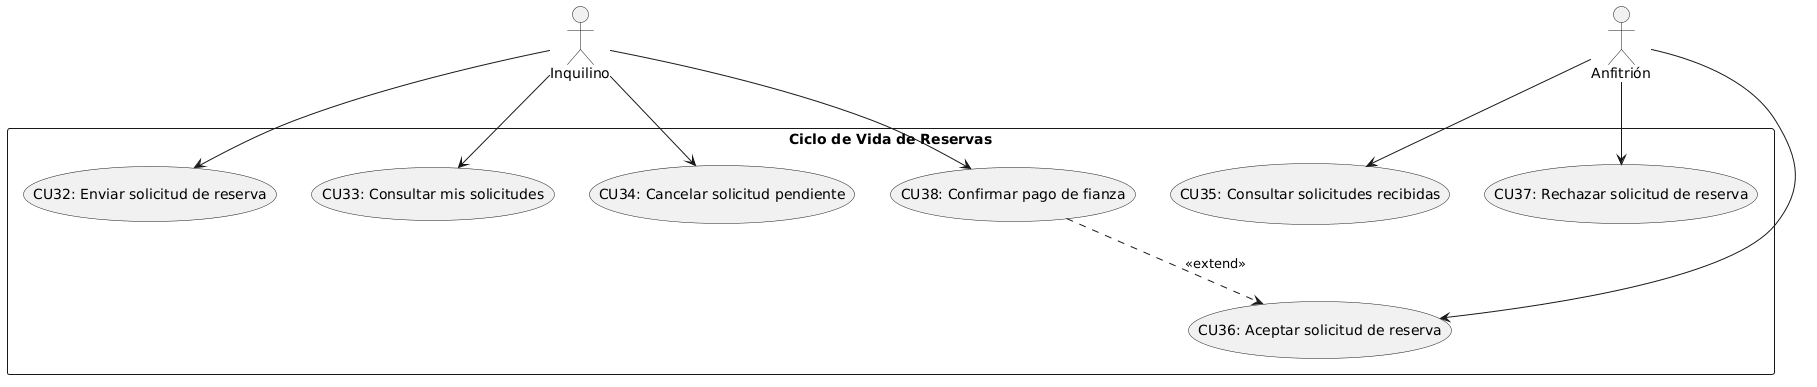
\includegraphics[width=0.75\textwidth]{AnalisisFuncional/img/dcu_reservas.png}
    \caption{Diagrama de casos de uso del ciclo de vida de reservas}
    \label{fig:dcu_reservas}
\end{figure}

    Las fichas descriptivas del ciclo de reserva comprenden desde CU32 hasta CU38:

\begin{table}[H]
\centering
\begin{tabular}{|p{3.2cm}|p{11.3cm}|}
\hline
\textbf{Caso de Uso} & \textbf{CU32: Enviar solicitud de reserva con rango de fechas} \\ \hline
\textbf{Actores} & Inquilino \\ \hline
\textbf{Descripción} & Remite una propuesta de estancia vinculada a un anuncio seleccionando fecha de entrada y salida \\ \hline
\textbf{Precondiciones} & Estar autenticado en la plataforma y no ser el titular del alojamiento \\ \hline
\textbf{Flujo básico} & 
1. El inquilino selecciona las fechas deseadas desde el calendario del anuncio. \newline
2. El sistema comprueba que no existan reservas confirmadas en conflicto temporal. \newline
3. El inquilino redacta un mensaje introductorio y confirma la solicitud. \newline
4. El backend registra la reserva en estado pendiente y notifica al anfitrión. \\ \hline
\end{tabular}
\caption{Especificación del caso de uso CU32.}
\label{tab:cu32}
\end{table}

\begin{table}[H]
\centering
\begin{tabular}{|p{3.2cm}|p{11.3cm}|}
\hline
\textbf{Caso de Uso} & \textbf{CU33: Consultar historial de mis solicitudes} \\ \hline
\textbf{Actores} & Inquilino \\ \hline
\textbf{Descripción} & Muestra el listado de reservas solicitadas por el usuario clasificadas por su estado actual \\ \hline
\textbf{Precondiciones} & Disponer de una sesión activa como inquilino \\ \hline
\textbf{Flujo básico} & 
1. El inquilino accede a su panel de reservas personales. \newline
2. El sistema recupera el registro de solicitudes (pendientes, aceptadas, rechazadas y finalizadas). \newline
3. La interfaz presenta los resúmenes económicos, fechas pactadas y accesos directos. \\ \hline
\end{tabular}
\caption{Especificación del caso de uso CU33.}
\label{tab:cu33}
\end{table}

\begin{table}[H]
\centering
\begin{tabular}{|p{3.2cm}|p{11.3cm}|}
\hline
\textbf{Caso de Uso} & \textbf{CU34: Cancelar solicitud de reserva pendiente} \\ \hline
\textbf{Actores} & Inquilino \\ \hline
\textbf{Descripción} & Permite al inquilino revocar una propuesta antes del pronunciamiento del anfitrión \\ \hline
\textbf{Precondiciones} & Que la reserva se encuentre formalmente en estado pendiente de aprobación \\ \hline
\textbf{Flujo básico} & 
1. El inquilino selecciona la solicitud pendiente y confirma la revocación. \newline
2. El sistema conmuta el estado de la reserva a cancelada. \newline
3. El backend libera el bloqueo preventivo del calendario y remite aviso al propietario. \\ \hline
\end{tabular}
\caption{Especificación del caso de uso CU34.}
\label{tab:cu34}
\end{table}

\begin{table}[H]
\centering
\begin{tabular}{|p{3.2cm}|p{11.3cm}|}
\hline
\textbf{Caso de Uso} & \textbf{CU35: Consultar solicitudes recibidas} \\ \hline
\textbf{Actores} & Anfitrión \\ \hline
\textbf{Descripción} & Despliega las peticiones de estancia pendientes de resolución para los alojamientos del propietario \\ \hline
\textbf{Precondiciones} & Ser titular de al menos un anuncio publicado \\ \hline
\textbf{Flujo básico} & 
1. El anfitrión accede a la bandeja de gestión de solicitudes entrantes. \newline
2. El sistema recupera las peticiones pendientes con el perfil del demandante y su historial. \newline
3. La interfaz expone los detalles temporales y económicos para facilitar la toma de decisión. \\ \hline
\end{tabular}
\caption{Especificación del caso de uso CU35.}
\label{tab:cu35}
\end{table}

\begin{table}[H]
\centering
\begin{tabular}{|p{3.2cm}|p{11.3cm}|}
\hline
\textbf{Caso de Uso} & \textbf{CU36: Aceptar solicitud de reserva} \\ \hline
\textbf{Actores} & Anfitrión \\ \hline
\textbf{Descripción} & Admite formalmente la estancia de un inquilino para el rango de fechas pactado \\ \hline
\textbf{Precondiciones} & Que la solicitud se encuentre en estado pendiente y el calendario disponible \\ \hline
\textbf{Flujo básico} & 
1. El anfitrión examina la petición y pulsa sobre la opción de confirmación. \newline
2. El backend bloquea de forma definitiva las fechas en el calendario del inmueble. \newline
3. El sistema actualiza el estado a aceptada y remite notificación al inquilino. \\ \hline
\end{tabular}
\caption{Especificación del caso de uso CU36.}
\label{tab:cu36}
\end{table}

\begin{table}[H]
\centering
\begin{tabular}{|p{3.2cm}|p{11.3cm}|}
\hline
\textbf{Caso de Uso} & \textbf{CU37: Rechazar solicitud de reserva} \\ \hline
\textbf{Actores} & Anfitrión \\ \hline
\textbf{Descripción} & Deniega una propuesta de estancia detallando de forma opcional el motivo de desestimación \\ \hline
\textbf{Precondiciones} & Que la reserva figure en estado pendiente \\ \hline
\textbf{Flujo básico} & 
1. El anfitrión selecciona la acción de desestimación en la solicitud correspondiente. \newline
2. El anfitrión introduce el motivo de desestimación si lo estima oportuno. \newline
3. El sistema marca la reserva en estado rechazada y actualiza el panel del inquilino. \\ \hline
\end{tabular}
\caption{Especificación del caso de uso CU37.}
\label{tab:cu37}
\end{table}

\begin{table}[H]
\centering
\begin{tabular}{|p{3.2cm}|p{11.3cm}|}
\hline
\textbf{Caso de Uso} & \textbf{CU38: Confirmar y registrar pago de fianza} \\ \hline
\textbf{Actores} & Inquilino \\ \hline
\textbf{Descripción} & Registra el abono del depósito de garantía exigido por el anfitrión para consolidar el contrato \\ \hline
\textbf{Precondiciones} & Que la solicitud de reserva haya sido aceptada previamente por el anfitrión \\ \hline
\textbf{Flujo básico} & 
1. El inquilino accede a su reserva aceptada y pulsa la opción de pago de fianza. \newline
2. El sistema presenta el desglose del importe del depósito establecido. \newline
3. El inquilino introduce los datos de transacción y formaliza la operación. \newline
4. El backend convalida la operación, emite comprobante y consolida la reserva como afianzada. \\ \hline
\end{tabular}
\caption{Especificación del caso de uso CU38.}
\label{tab:cu38}
\end{table}